\documentclass[../main.tex]{subfiles}
\graphicspath{{\subfix{../images/}}}
\begin{document}

Let's consider a general MLP consisting of $m$ neurons in the input, $d$ neurons
in the hidden, and $t$ neurons in the output layers:

%General MLP picture
\begin{center}
    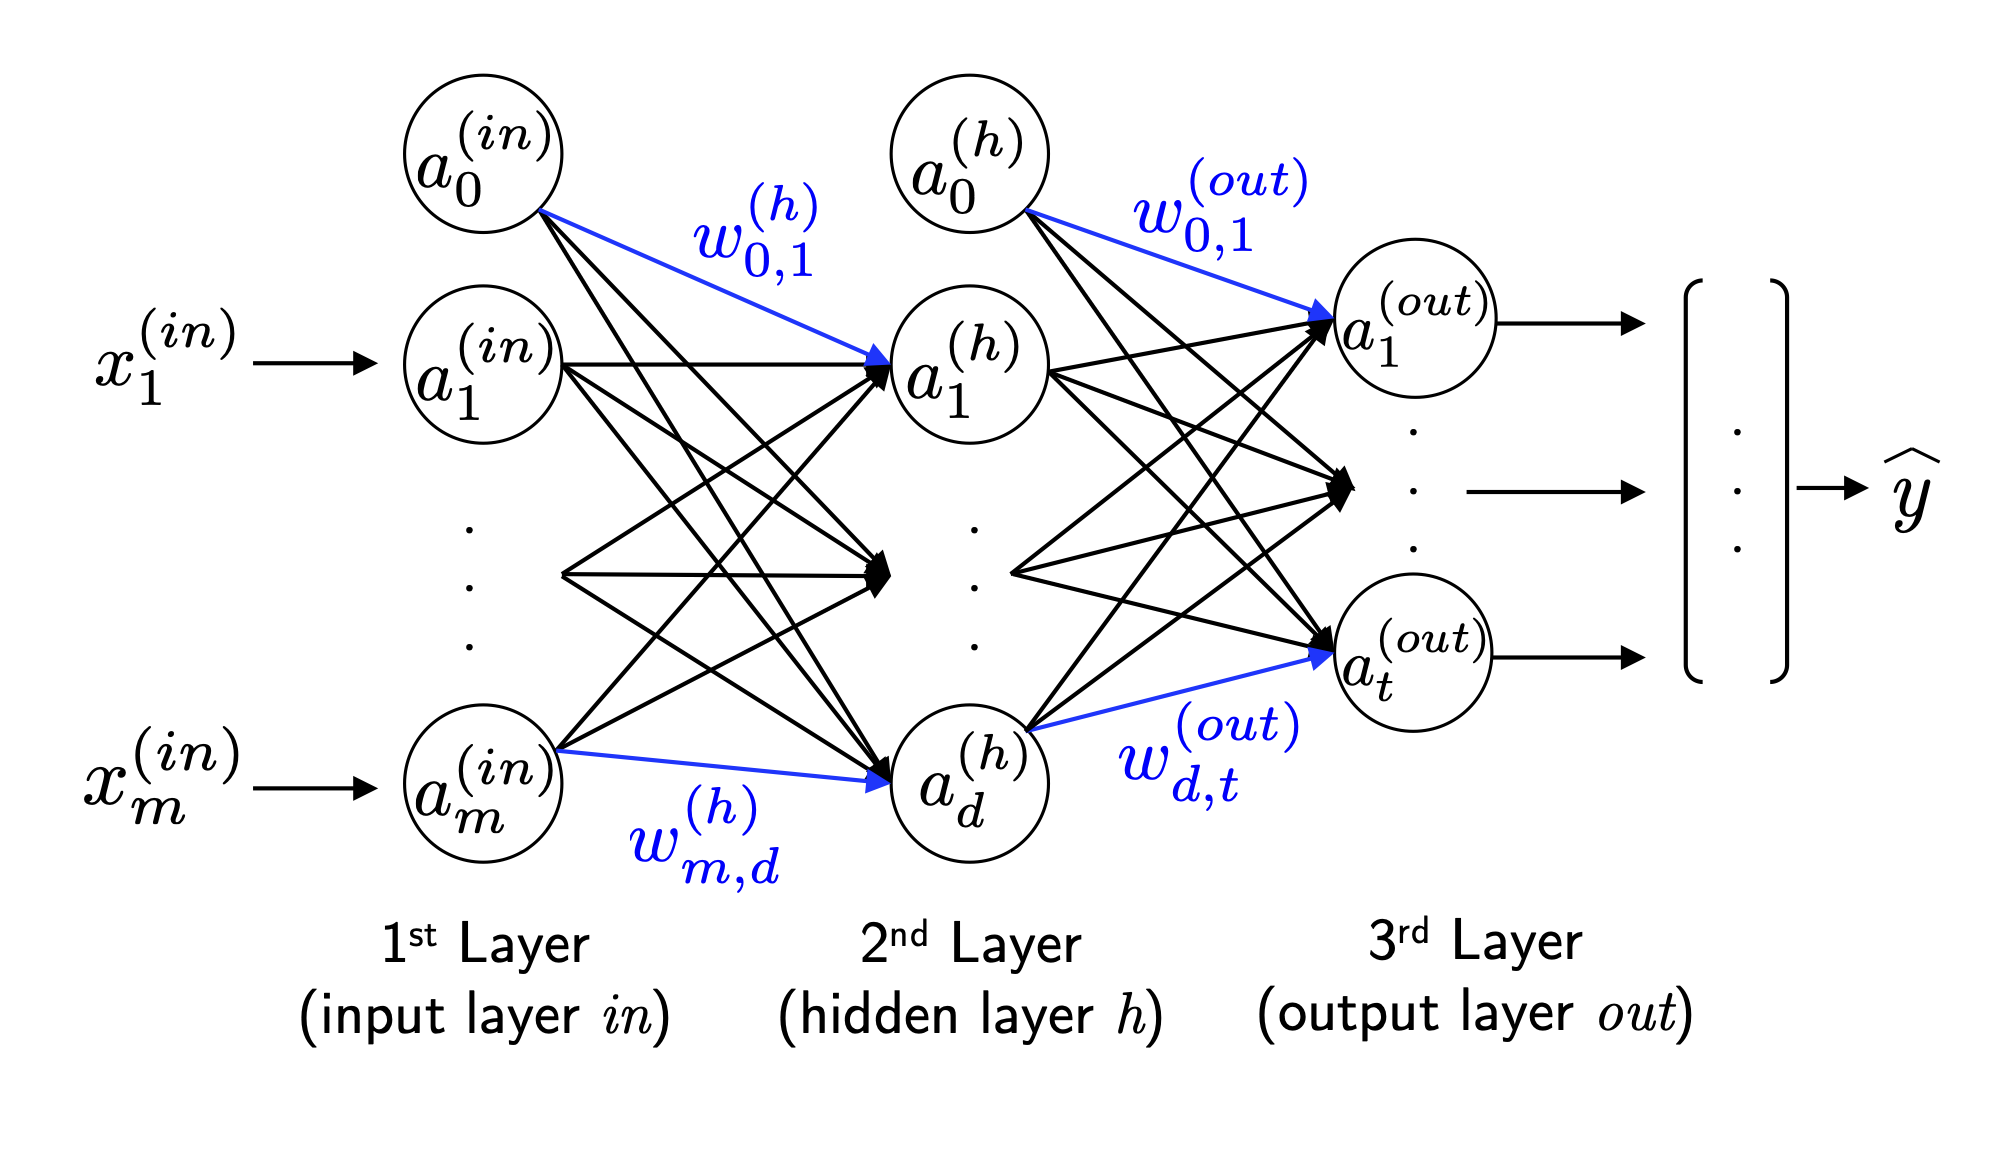
\includegraphics[width = 16cm, height = 9cm]{1.png}
\end{center}

Also, let's imagine ONE training example goes through the network. This is
to what its journey looks like from the input layer to the output layer:

\pagebreak
\[[a_0^{(in)}, a_1^{(in)}, a_2^{(in)}, \cdots, a_m^{(in)}]\]
\[\downarrow\]
\[W^{(h)}\]
\[\downarrow\]                  
\[[z_1^{(h)}, z_2^{(h)}, \cdots, z_d^{(h)}]\]
\[\downarrow\]
\[\phi(\bullet)\]
\[\downarrow\]
\[[a_0^{(h)}, a_1^{(h)}, a_2^{(h)}, \cdots, a_d^{(h)}]\]
\[\downarrow\]
\[W^{(out)}\]
\[\downarrow\]                  
\[[z_1^{(out)}, z_2^{(out)}, \cdots, z_t^{(out)}]\]
\[\downarrow\]
\[\phi(\bullet)\]
\[\downarrow\]
\[[a_1^{(out)}, a_2^{(out)}, \cdots, a_t^{(out)}]\]

\vspace{5mm} %5mm vertical space

\emph{Note: I represent training examples and weight vectors as row vectors}

\vspace{5mm} %5mm vertical space

With that out of the way, let's come back to our original purpose: Deriving the
formula Dr. Raschka used. This document is concerned with $W^{(out)}$ 
(the weights between the hidden and output layer). In the following three sections,
I will manually derive the gradients.

\vspace{5mm} %5mm vertical space

Let's first consider \underline{ONE} training example, then expand to $n$ examples.

%Insert picture here.
\end{document}